Aside from the BDT based multivariate technique, we also employ a Matrix Element technique~\cite{MENote}. 
This method has already been used in top quark mass and cross-section 
measurements, the discovery of single top production, and Higgs boson searches at the Tevatron.  
The Matrix Element method works by calculating the probability for each recorded
event to originate from a specific physics process.
This is done by comparing the differential cross sections predicted by Matrix Element 
calculations for the signal and background processes given the kinematic observables
on an event-by-event basis.
The discriminating power arises because the differential cross sections for 
signal and background events are largest in different regions of the available
kinematic phase space. 

One complication of the Higgs to $WW$ leptonic final state is that it is not fully 
reconstructed, with two neutrinos in the final state. 
Information about the $z$-components of the neutrino momenta as well as the individual 
neutrino transverse components are missing. It is therefore necessary to integrate 
over these unknown quantities, which we perform using the importance sampling 
integration method.
The Matrix Element functions used in the determination of the differential cross sections
for this analysis are obtained from  MCFM v6.2.  While MCFM 
provides both leading order (LO) and next-to leading (NLO) cross-section calculations for 
some relevant background and Higgs processes in $pp$ collisions, only the
LO is currently used.

The probabilities for all processes under consideration are combined 
to construct a single discriminant, called the Likelihood Ratio ($LR$).  
To construct the optimal discriminant, one should calculate 
event probabilities for all of the background processes. In reality, however, having 
probabilities for the signal hypothesis and the main backgrounds is sufficient for the 
desired level of discrimination. In this analysis we calculate event probabilities 
for gluon fusion Higgs boson production ($ggH$), electroweak $q\bar{q}\rightarrow WW$ pair 
production ($WW$) and the $W+jet$ process where a $W$ boson is produced in association with one hadronic jet. 


\subsection{Event Probability Calculation}

In the Matrix Element technique we calculate a probability  for each event assuming a
certain hypothesis.  The probability is denoted by $P(x_{obs};\alpha)$,
where $\alpha$ is a set of physics 
parameters of the specific model and $x_{obs}$ are the measured kinematic quantities.
In the case of Standard Model Higgs Boson production,
 $\alpha$ is $(m_H, \Gamma_H)$, where  $m_H$ is the Higgs mass 
and $\Gamma_H$ is the Higgs width. There are eight observables, $x_{obs}$, representing all the 
lepton kinematic information: lepton momenta $\vec{l}^+$, $\vec{l}^-$ and missing 
transverse momentum, \met$_x$ and \met$_y$.

It should be noted that additional information such as the number of jets
produced and the total visible energy might further differentiate the Higgs signal from SM
$WW$ production,
but they can suffer from significant  QCD uncertainties. For this reason we 
deliberately do not use hadronic information at all but use
only the kinematic information from the leptons and the missing $E_T$, indirectly
through the system boost (see below).

The event probability density is given by
\begin{equation}
P(x_{obs};\alpha) =
 \frac{1}{ < \sigma(\alpha) > }
 \int \frac {d \sigma_{0} (y;\alpha) }{ dy }
 \epsilon (y) G(x_{obs},y) dy,  
\label{eqn:EvtProb}  
\end{equation}
where $y$ denotes the true values of the observables,
$\frac{d \sigma_{LO}}{dy}$ is the  parton-level differential cross-section differential
in those observables, $\epsilon(y)$ is the detector acceptance and efficiency function
and $G(x_{obs},y)$ is the transfer function between the true and measured values of the
observables, representing the detector resolution.
Equation (\ref{eqn:EvtProb}) integrates over all possible true values of the
observables, $y$, consistent with the measured quantities $x_{obs}$.
The constant $<\sigma(\alpha)>$ normalizes the total event probability to unity

The efficiency function is the probability for a parton-level object with momentum 
$p$ to be reconstructed as a lepton with momentum $q$. The lepton efficiency is parameterized 
as a function of transverse momentum and pseudo-rapidity and extracted from $WW$ Monte Carlo. 
Note that the efficiency function in Equation~\ref{eqn:EvtProb} can be factorized out of
the integral when calculating event probabilities.
The lepton momenta are smeared according to the measured lepton mometum resolutions. 

Treatment of the $W+jet$ event probability calculation deserves special discussion.
For these events to be reconstructed in the dilepton final state,
one of the reconstructed leptons has been faked by a parton fragmenting and hadronizing 
into a QCD jet which then fakes the signature of a lepton in the detector. To account for this 
effect properly, we multiply the differential cross-section for the $W+jet$ process by the 
probability for a parton to be reconstructed as a lepton with the measured kinematics. 
This probability can be factorized into two terms:
\begin{eqnarray}
\begin{array}{lcl}
P(parton\rightarrow lepton)=P(parton\rightarrow FO)\times P(FO\rightarrow lepton)
\end{array} 
\end{eqnarray} 
where FO refers to a so-called "fakeable object" (see Sec.~\ref{sec:bkg_fakes}). 
The first term in the product is measured using Monte Carlo and parametrized
in $p_{T}$ and $\eta$.  The second term is the fake rate measured in the data 
(see Sec.~\ref{sec:bkg_fakes}).
We verify the $P(parton\rightarrow lepton)$ values we obtain from this method by 
comparing them to ones measured in a $\gamma+jet$ Monte Carlo sample and $\gamma+jet$ data.
The probabilities agree within the uncertainty of $30\%$.  

One final complication that must be considered is the boost of the initial state. 
In the leading order Matrix Element calculation there is no initial state radiation. 
To account for the transverse recoil and thus improve the performance of our discriminant
on data, we integrate over the possible values of the system boost $k_{T}(k_{x},k_{y})$. 
The $k_T$ model is extracted for each jet bin from Monte Carlo for each process separately. 

\subsection{Likelihood Ratio Discriminator}
Event probabilities, calculated as described above, are used to construct 
a likelihood ratio discriminant which we use in a one-dimensional template fit, defined as:
\begin{equation}
\label{eqn:LR}
LR = \frac { P_s} { P_s + \sum_i k_{bi} P_{bi}},
\end{equation}
where $P_s$  is the probability for the signal, $P_{bi}$ is the probability for background
process $i$, and
$k_{bi}$ is the expected fractional contribution of background $i$,
satisfying the sum $\sum k_{bi} =1$.
Because signal events are expected to have $P_s>P_b$ and vice-versa for background events, 
the value of $LR$ is close to one for signal and zero for background processes.
The calculation of $P_s$ is a function of Higgs mass, so the likelihood ratio
shape depends on $m_H$. This is true for both signal and background templates of $LR$. 

\subsection{\texorpdfstring{Results with $\intlumiEightTeV$}{Results on data}}

Figures~~\ref{fig:me_lr_115_120},~\ref{fig:me_lr_130_140},
~\ref{fig:me_lr_130_140} and~~\ref{fig:me_lr_160_200} show the matrix element output 
distributions, comparing data and MC for several higgs mass hypotheses. We then perform the 
shape analysis based on these output in the same way as in the BDT based shape analysis. 
The same treatment of the shape variations are applied as well. 

The expected and observed upper limits at 95\%C.L. for each mass point are shown in Table~\ref{tab:limits_me_5fb_0j} 
and Figure~\ref{fig:limits_me_5fb} for the dataset corresponding to $\intlumiEightTeV$. 
The sensitivity performance of the matrix element method are
consistent with the BDT-based approach shown in Section~\ref{app:appendix_limits_bychannel}.

%%%%%%%%%%%%%%%%%%%%%%%%%%%%%%
\begin{figure}[!hbtp]
\centering
\subfigure[ME 0-Jet OF]{
\label{subfig:me_0jof}
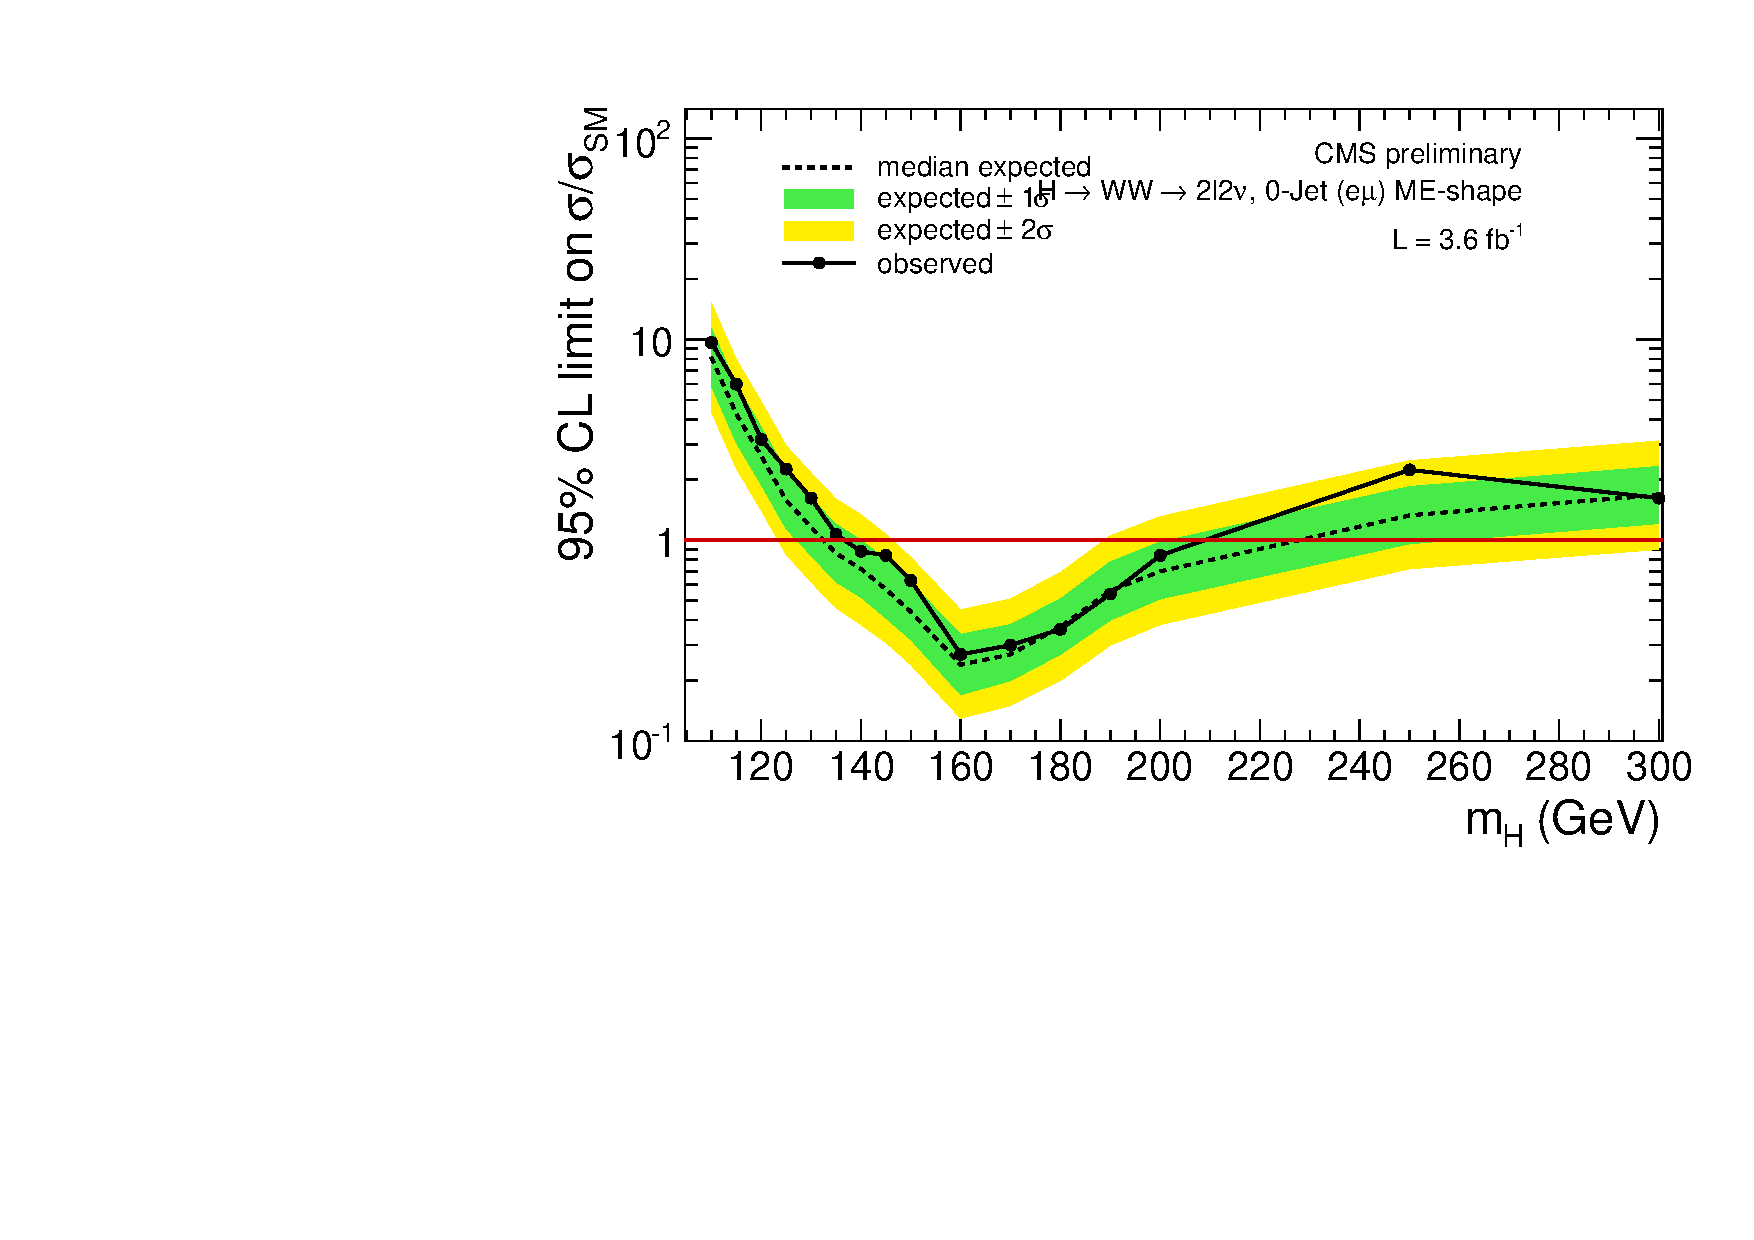
\includegraphics[width=.45\textwidth]{figures/limits_0jof_shape_me-CLs-asymptotic_zoom_log.pdf}
}
\centering
\subfigure[ME 0-Jet SF]{
\label{subfig:me_0jsf}
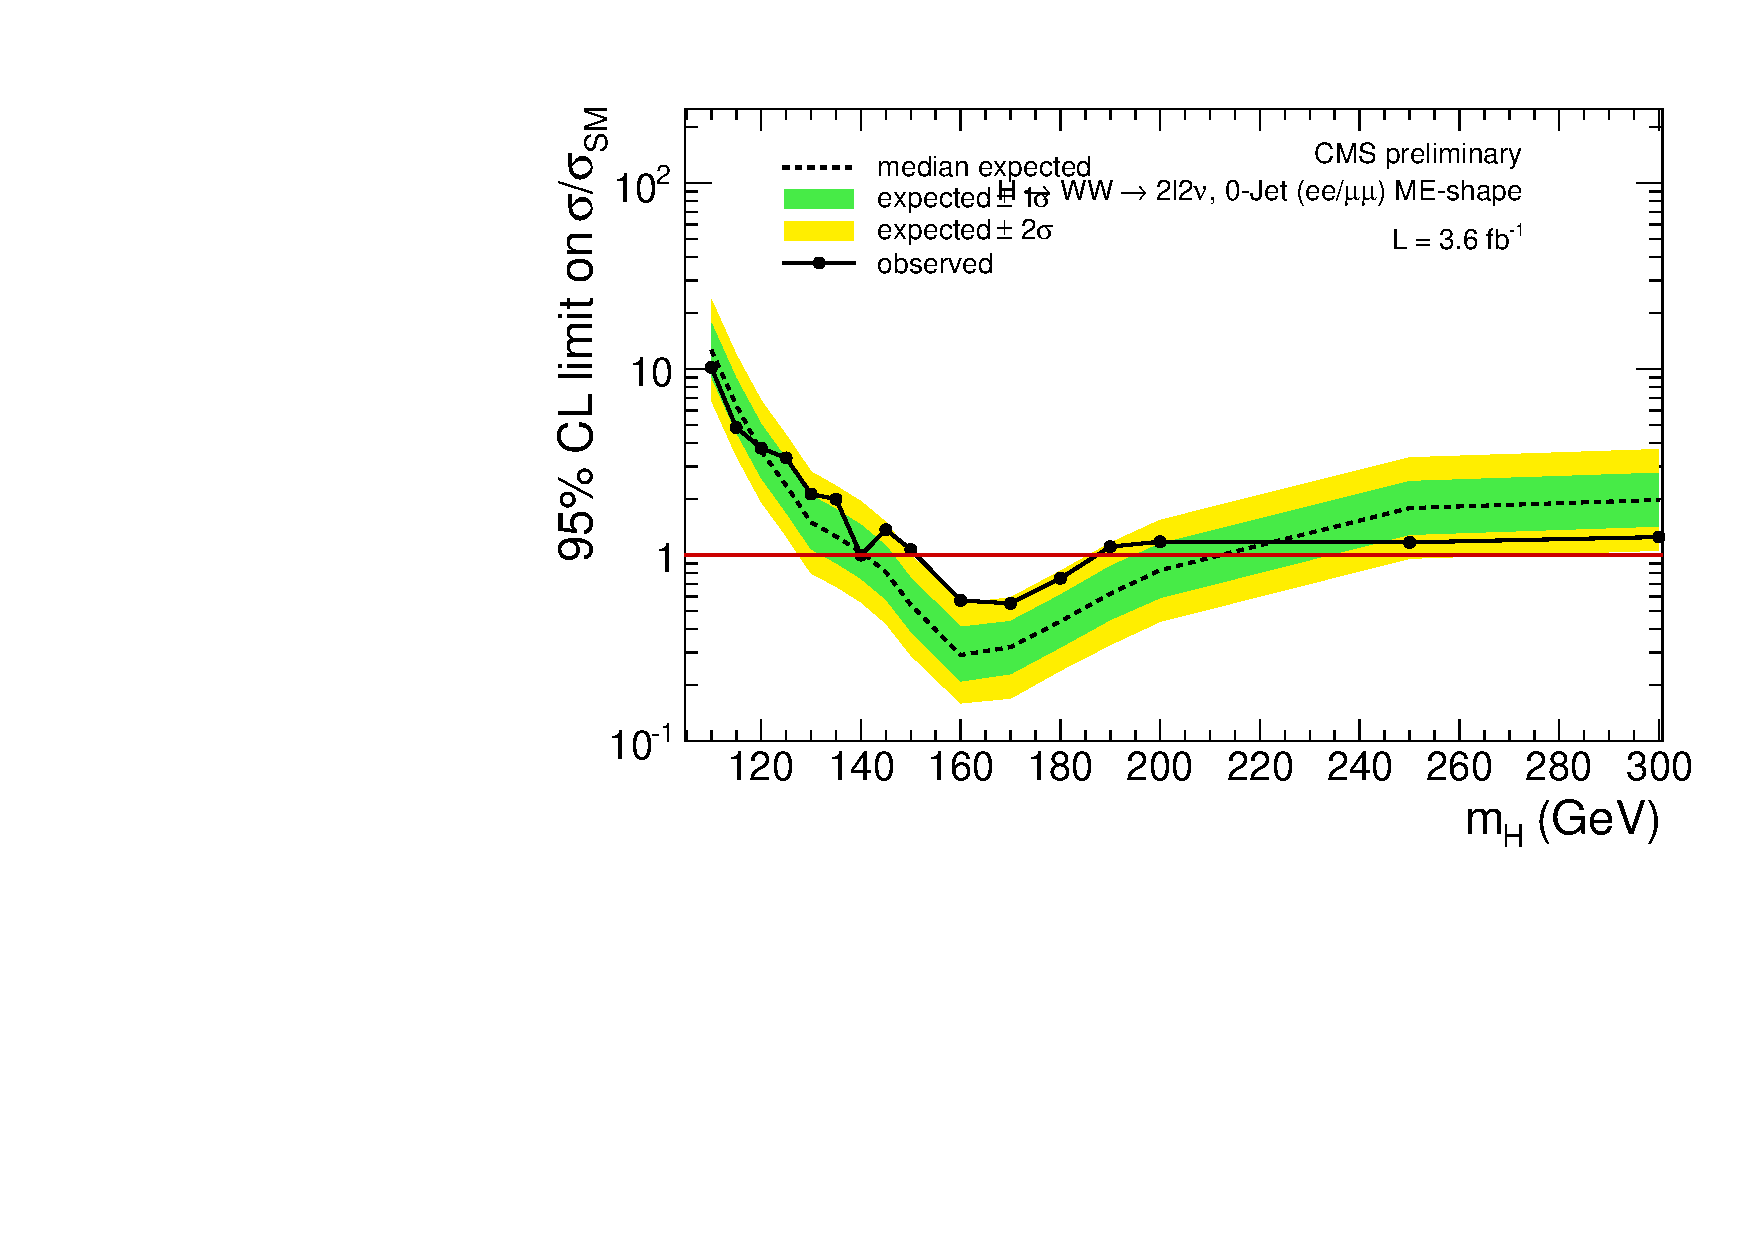
\includegraphics[width=.45\textwidth]{figures/limits_0jsf_shape_me-CLs-asymptotic_zoom_log.pdf}
}\\
\centering
\subfigure[ME 0-Jet combined]{
\label{subfig:me_0j}
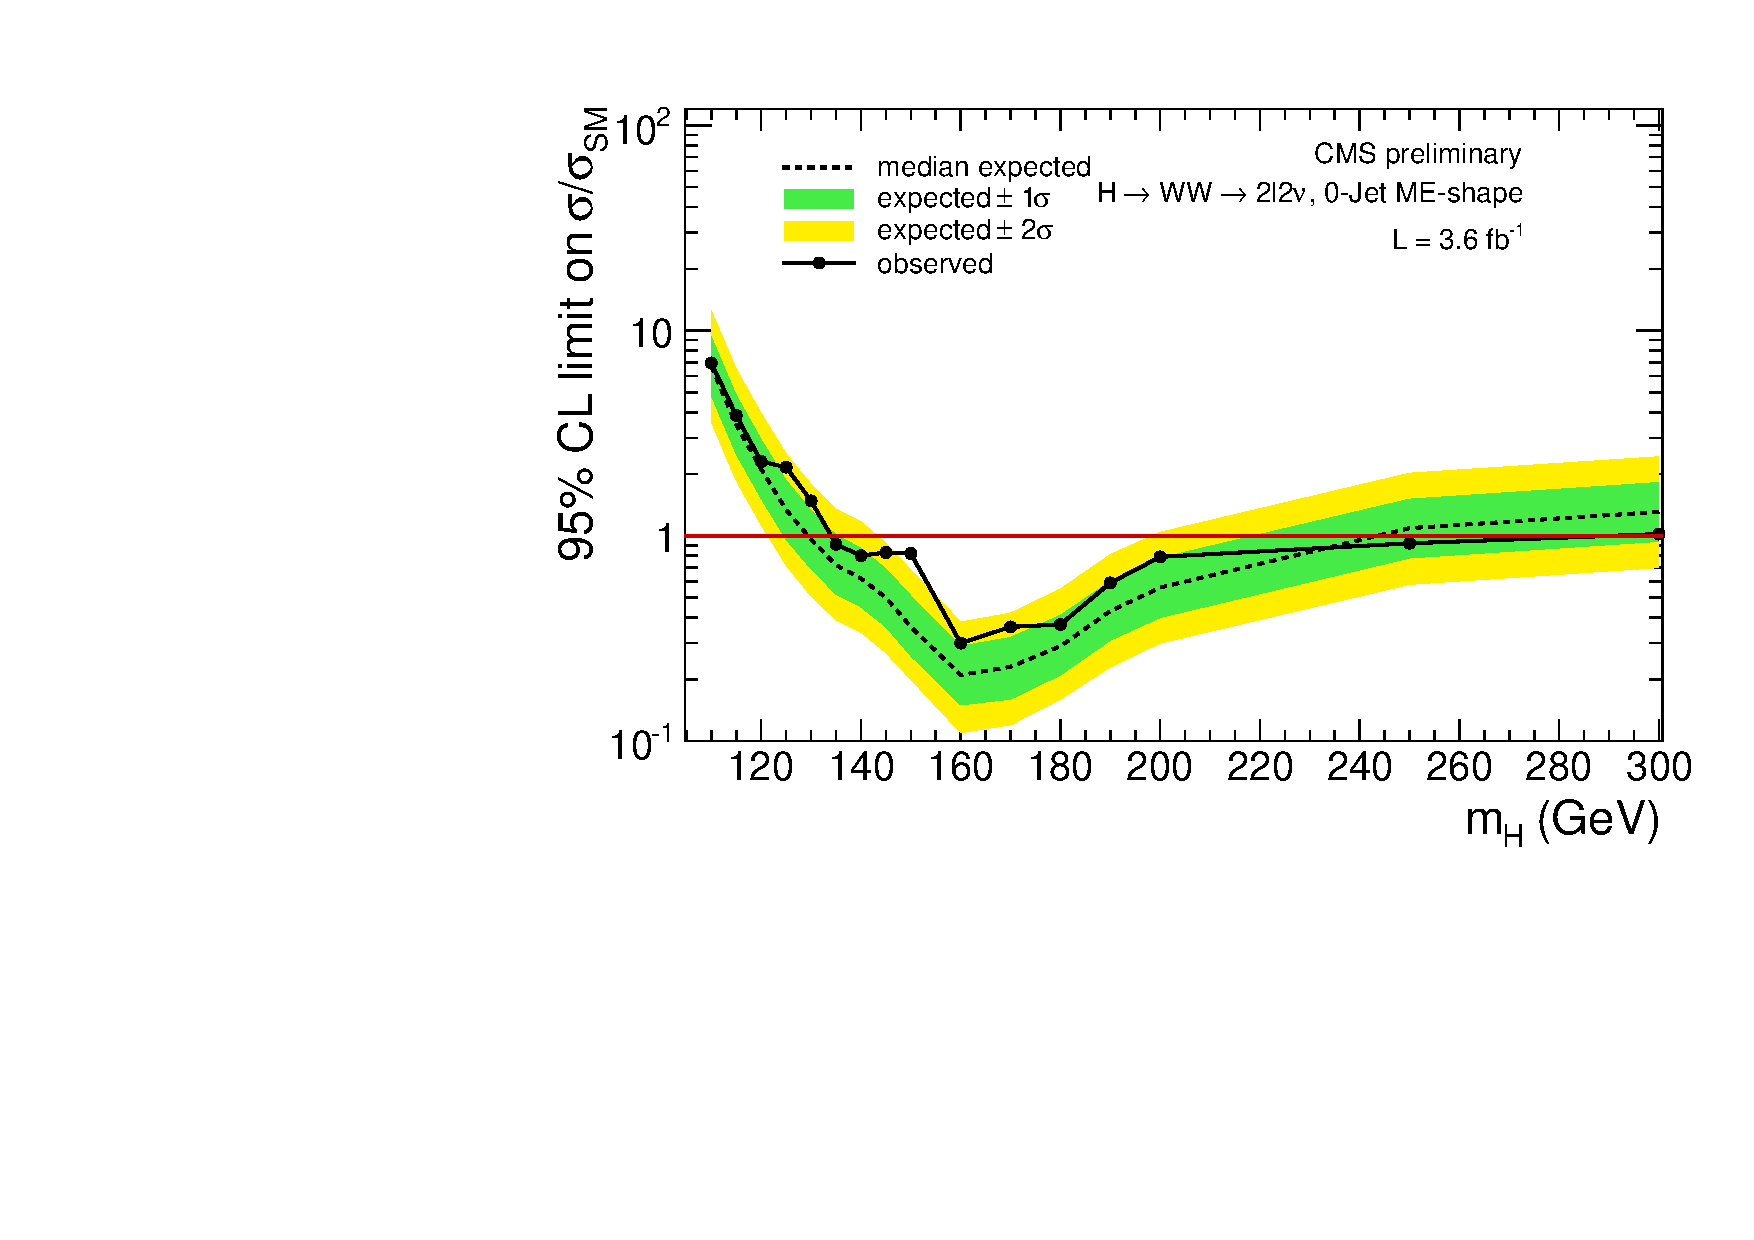
\includegraphics[width=.45\textwidth]{figures/limits_0j_shape_me-CLs-asymptotic_zoom_log.pdf}
}
\caption{ Shape analysis upper limits based on the matrix element outputs at 95\% C.L. for $\intlumiEightTeV$ data. }
\label{fig:limits_me_5fb}
\end{figure}
%%%%%%%%%%%%%%%%%%%%%%%%%%%%%%

%%%%%%%%%%%%%%%%%%%%%%%%%%%%%%
\begin{table}
\begin{center}
\begin{tabular}{c c c c c c}
\hline\hline
 Higgs Mass   & Observed & Median expected & Expected range for 68\% & Expected range for 95\%   \\
\hline
\multicolumn{5}{c} {0-Jet} \\
\hline
110 & 7.0 & 6.7 & [4.8, 9.3] & [3.6, 12.5] \\
115 & 3.9 & 3.5 & [2.5, 4.8] & [1.9, 6.5] \\
120 & 2.3 & 2.1 & [1.5, 2.9] & [1.1, 3.9] \\
125 & 2.2 & 1.3 & [1.0, 1.9] & [0.7, 2.5] \\
130 & 1.5 & 1.0 & [0.7, 1.3] & [0.5, 1.8] \\
135 & 0.9 & 0.7 & [0.5, 1.0] & [0.4, 1.4] \\
140 & 0.8 & 0.6 & [0.5, 0.9] & [0.3, 1.2] \\
145 & 0.8 & 0.5 & [0.4, 0.7] & [0.3, 0.9] \\
150 & 0.8 & 0.4 & [0.3, 0.5] & [0.2, 0.7] \\
160 & 0.3 & 0.2 & [0.1, 0.3] & [0.1, 0.4] \\
170 & 0.4 & 0.2 & [0.2, 0.3] & [0.1, 0.4] \\
180 & 0.4 & 0.3 & [0.2, 0.4] & [0.2, 0.5] \\
190 & 0.6 & 0.4 & [0.3, 0.6] & [0.2, 0.8] \\
200 & 0.8 & 0.6 & [0.4, 0.8] & [0.3, 1.0] \\
\hline
\multicolumn{5}{c} {0-Jet bin OF} \\
\hline
110 & 9.6 & 8.2 & [5.9, 11.3] & [4.4, 15.2] \\
115 & 6.0 & 4.2 & [3.1, 5.9] & [2.3, 7.9] \\
120 & 3.2 & 2.6 & [1.9, 3.7] & [1.4, 4.9] \\
125 & 2.3 & 1.6 & [1.1, 2.2] & [0.8, 3.0] \\
130 & 1.6 & 1.2 & [0.8, 1.6] & [0.6, 2.2] \\
135 & 1.1 & 0.9 & [0.6, 1.2] & [0.5, 1.6] \\
140 & 0.9 & 0.7 & [0.5, 1.0] & [0.4, 1.3] \\
145 & 0.8 & 0.6 & [0.4, 0.8] & [0.3, 1.1] \\
150 & 0.6 & 0.4 & [0.3, 0.6] & [0.2, 0.8] \\
160 & 0.3 & 0.2 & [0.2, 0.3] & [0.1, 0.5] \\
170 & 0.3 & 0.3 & [0.2, 0.4] & [0.1, 0.5] \\
180 & 0.4 & 0.4 & [0.3, 0.5] & [0.2, 0.7] \\
190 & 0.5 & 0.6 & [0.4, 0.8] & [0.3, 1.0] \\
200 & 0.8 & 0.7 & [0.5, 1.0] & [0.4, 1.3] \\
\hline
\multicolumn{5}{c} {0-Jet bin SF} \\
\hline
110 & 10.2 & 12.7 & [9.1, 17.7] & [6.8, 23.7] \\
115 & 4.8 & 6.4 & [4.6, 8.9] & [3.4, 11.9] \\
120 & 3.8 & 3.6 & [2.6, 5.0] & [1.9, 6.8] \\
125 & 3.3 & 2.4 & [1.7, 3.3] & [1.3, 4.4] \\
130 & 2.1 & 1.5 & [1.1, 2.1] & [0.8, 2.8] \\
135 & 2.0 & 1.3 & [0.9, 1.8] & [0.7, 2.4] \\
140 & 1.0 & 1.0 & [0.7, 1.4] & [0.6, 1.9] \\
145 & 1.4 & 0.8 & [0.6, 1.1] & [0.4, 1.5] \\
150 & 1.1 & 0.5 & [0.4, 0.7] & [0.3, 1.0] \\
160 & 0.6 & 0.3 & [0.2, 0.4] & [0.2, 0.5] \\
170 & 0.5 & 0.3 & [0.2, 0.4] & [0.2, 0.6] \\
180 & 0.7 & 0.4 & [0.3, 0.6] & [0.2, 0.8] \\
190 & 1.1 & 0.6 & [0.4, 0.9] & [0.3, 1.2] \\
200 & 1.2 & 0.8 & [0.6, 1.1] & [0.4, 1.5] \\
\hline\hline
\end{tabular}
\end{center}
\caption{Expected and observed upper limits for SM Higgs using {\bf shape analysis based 
    on matrix element output} for $\intlumiEightTeV$ data the matrix element outputs 
  for the {\bf 0-jet} bin two sub-channels. }
\label{tab:limits_me_5fb_0j}
\end{table}
%%%%%%%%%%%%%%%%%%%%%%%%%%%%%%

\clearpage
\subsection{\texorpdfstring{Likelihood ratio distributionswith $\intlumiEightTeV$}{Likelihood ratio distributions}}

The likelihood ratio output is shown for the observed data and the background
predictions in Figures \ref{fig:me_lr_115_120}, \ref{fig:me_lr_130_140}, 
\ref{fig:me_lr_140_150} and \ref{fig:me_lr_160_200}.

%%%%%%%%%%%%%%%%%%%%%%        
\begin{figure}[!hbtp]
\centering
\subfigure[$mH=115 GeV$]{
\centering                    
\label{subfig:lr115}      
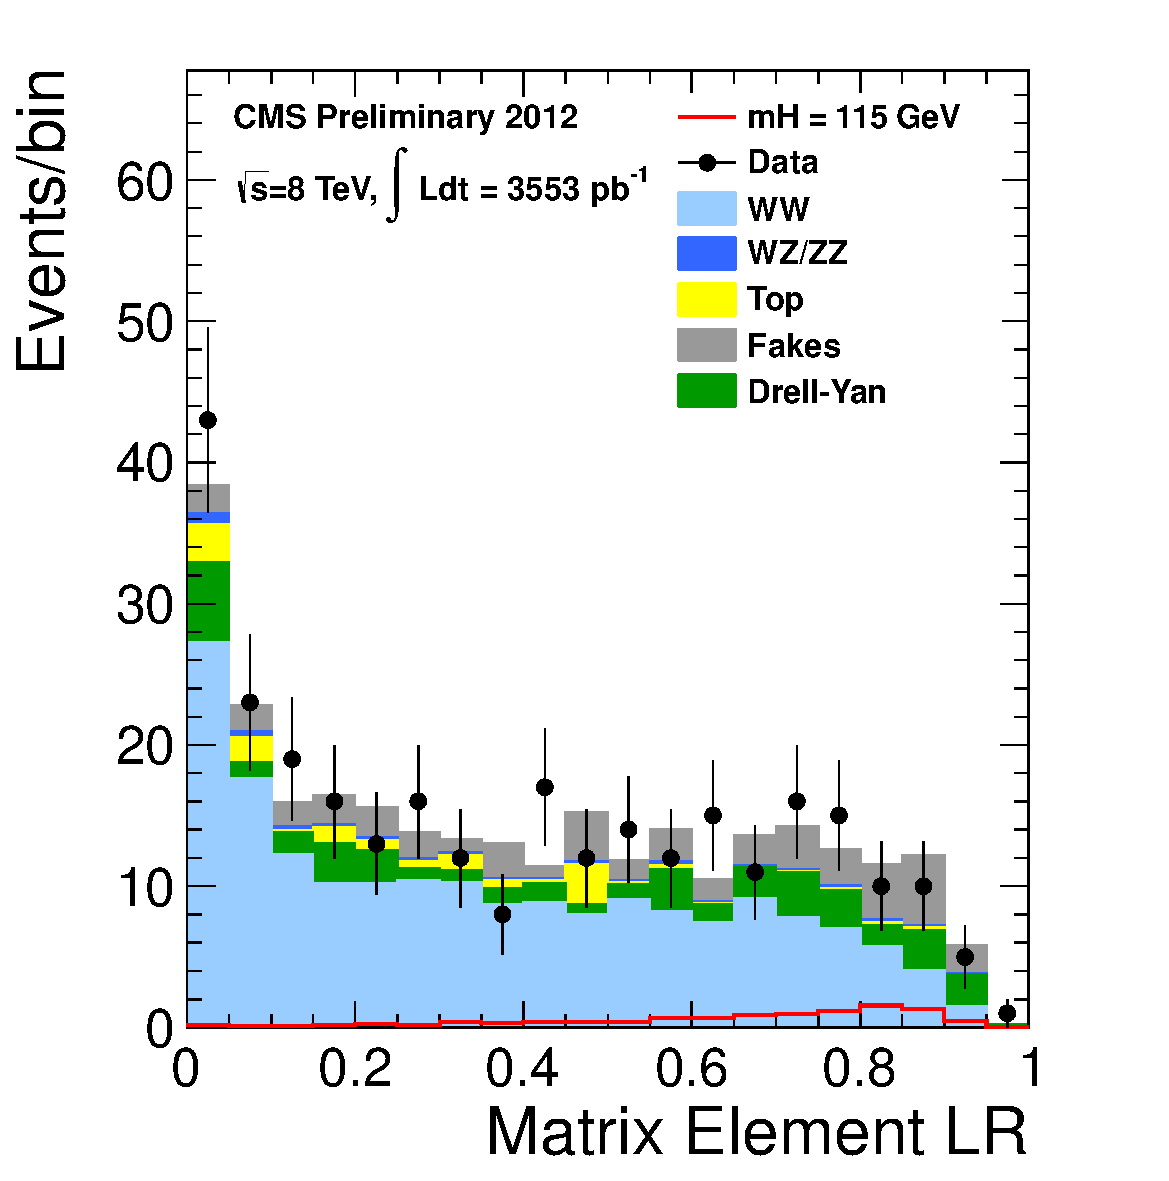
\includegraphics[width=.45\textwidth]{figures/hww_analysis19_115_lr_incl_0j.pdf}}
\subfigure[$mH=120 GeV$]{               
\centering
\label{subfig:lr120}      
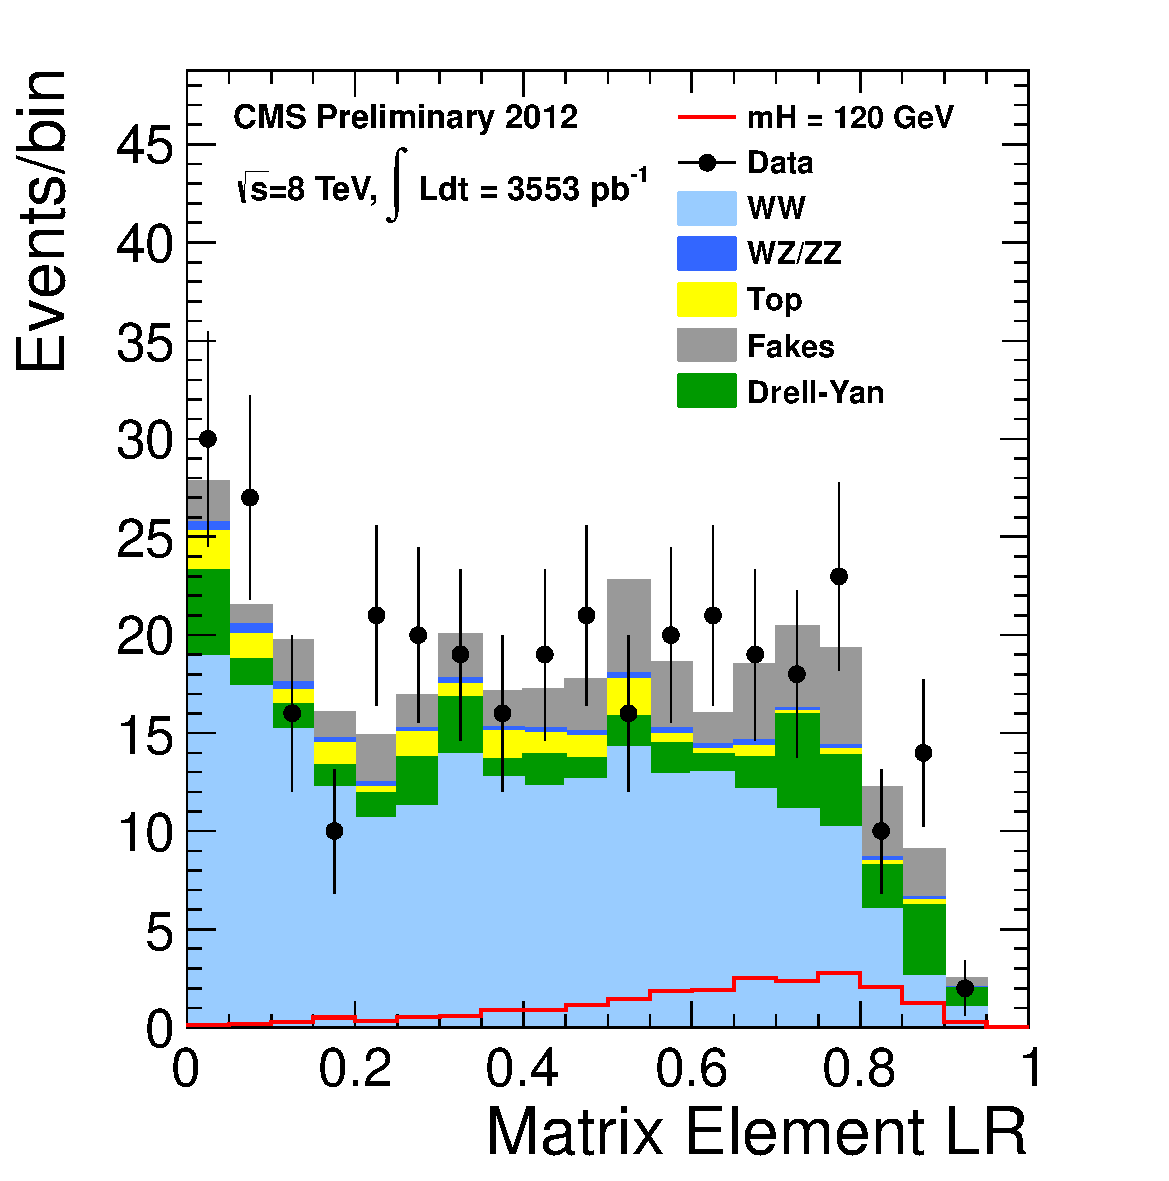
\includegraphics[width=.45\textwidth]{figures/hww_analysis19_120_lr_incl_0j.pdf}}
\caption{Likelihood ratio for Higgs mass hypotheses 115 and 120 \GeV.}
\label{fig:me_lr_115_120}
\end{figure}


\begin{figure}[!hbtp]
\centering
\subfigure[$mH=125 GeV$]{
\label{subfig:lr125}
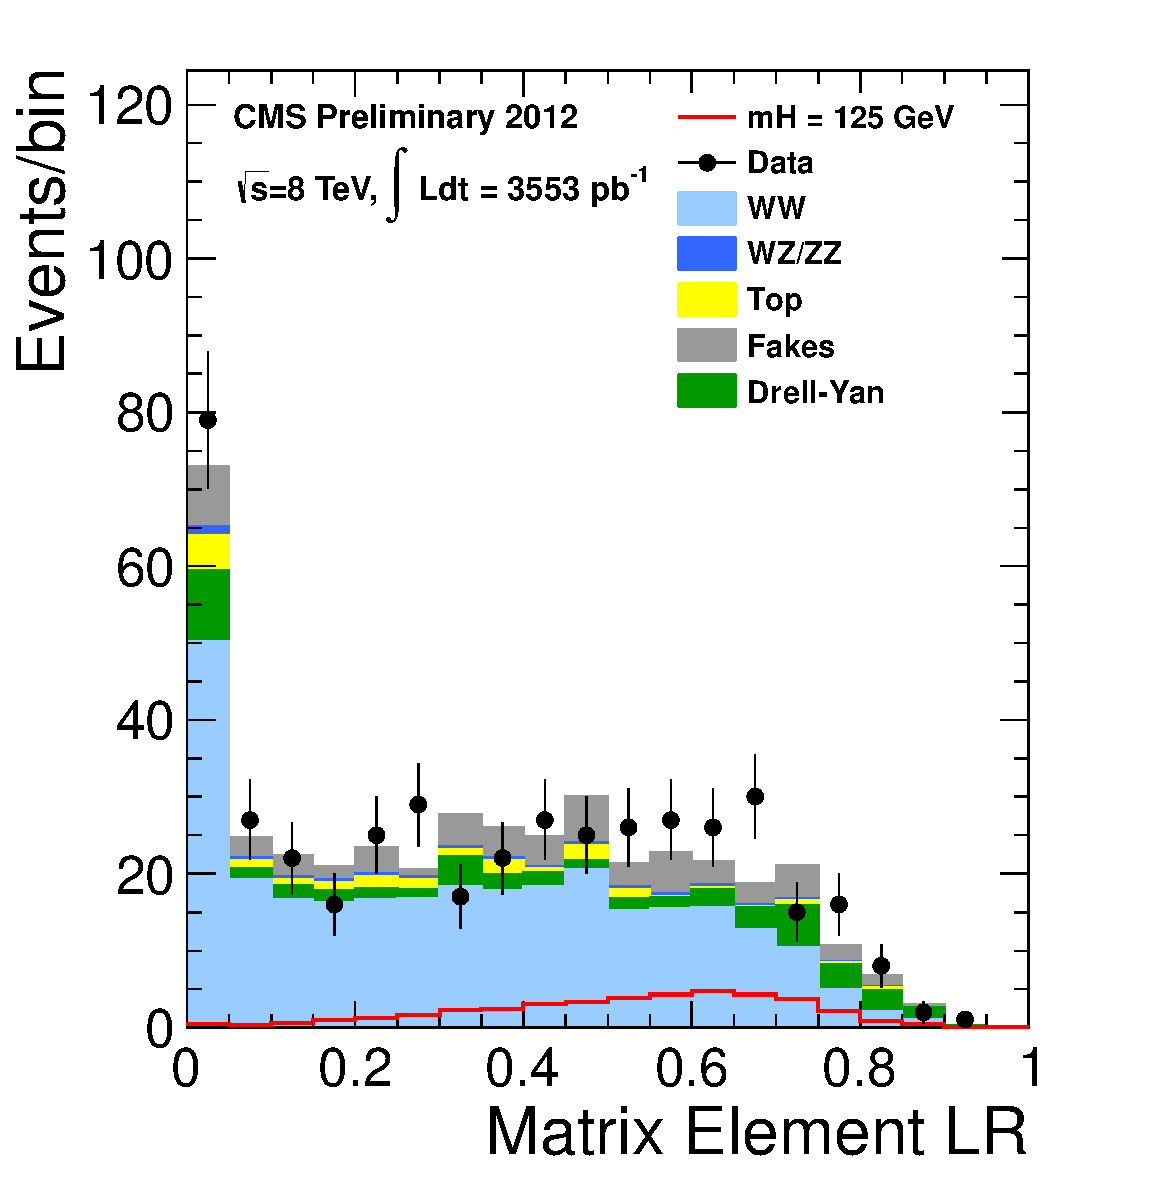
\includegraphics[width=.45\textwidth]{figures/hww_analysis19_125_lr_incl_0j.pdf}}
\subfigure[$mH=130 GeV$]{
\centering
\label{subfig:lr130}
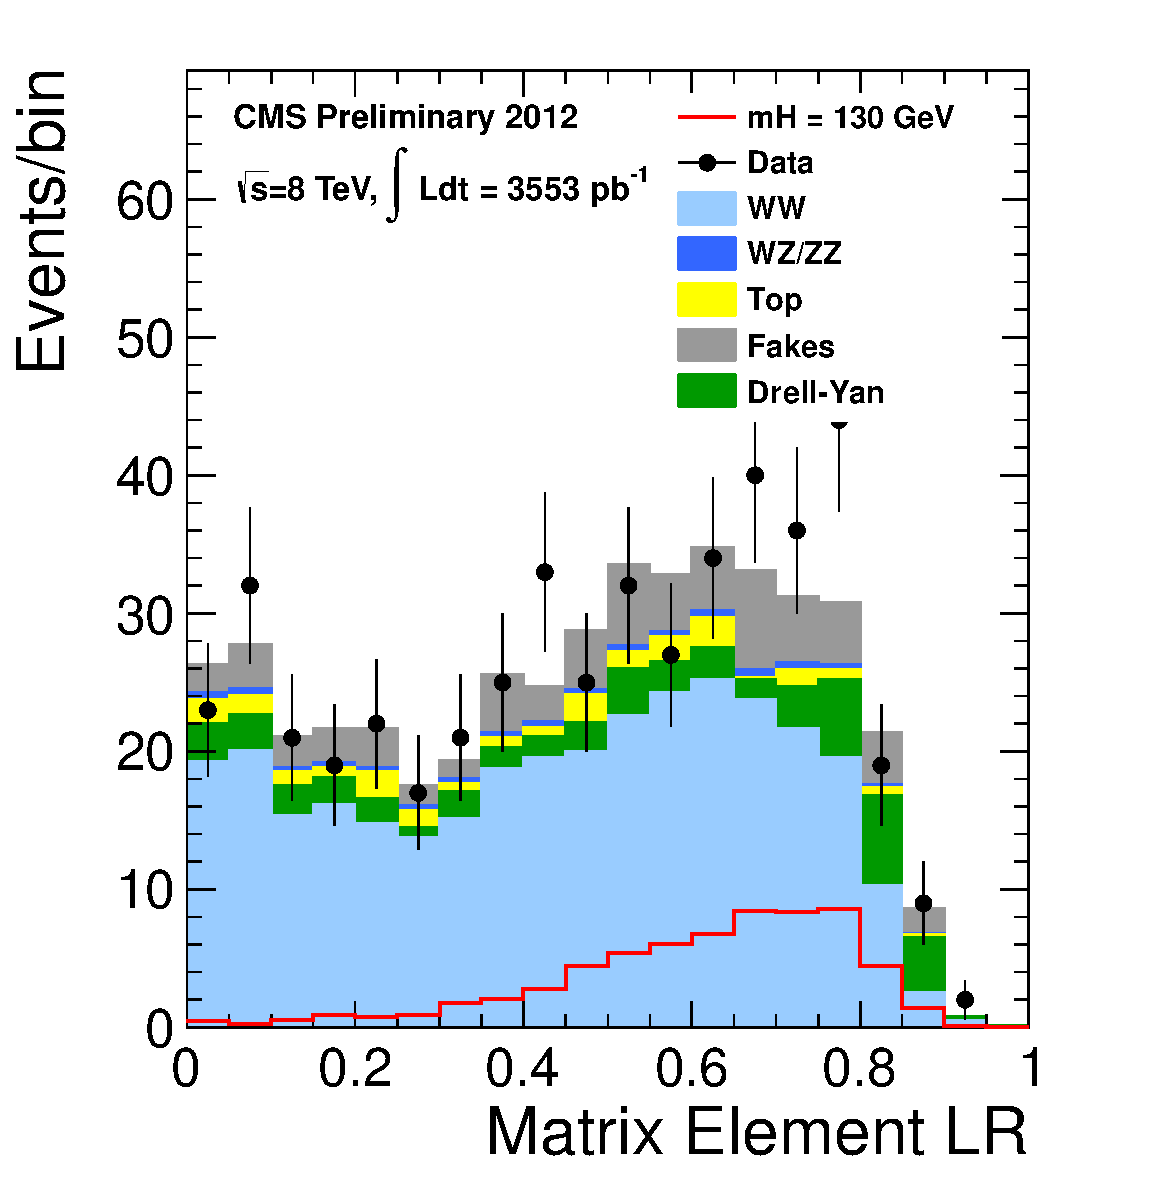
\includegraphics[width=.45\textwidth]{figures/hww_analysis19_130_lr_incl_0j.pdf}}
\caption{Likelihood ratio for Higgs mass hypotheses 125 and 130 \GeV.}
\label{fig:me_lr_130_140}
\end{figure}


\begin{figure}[!hbtp]
\subfigure[$mH=140 GeV$]{
\centering
\label{subfig:lr140}
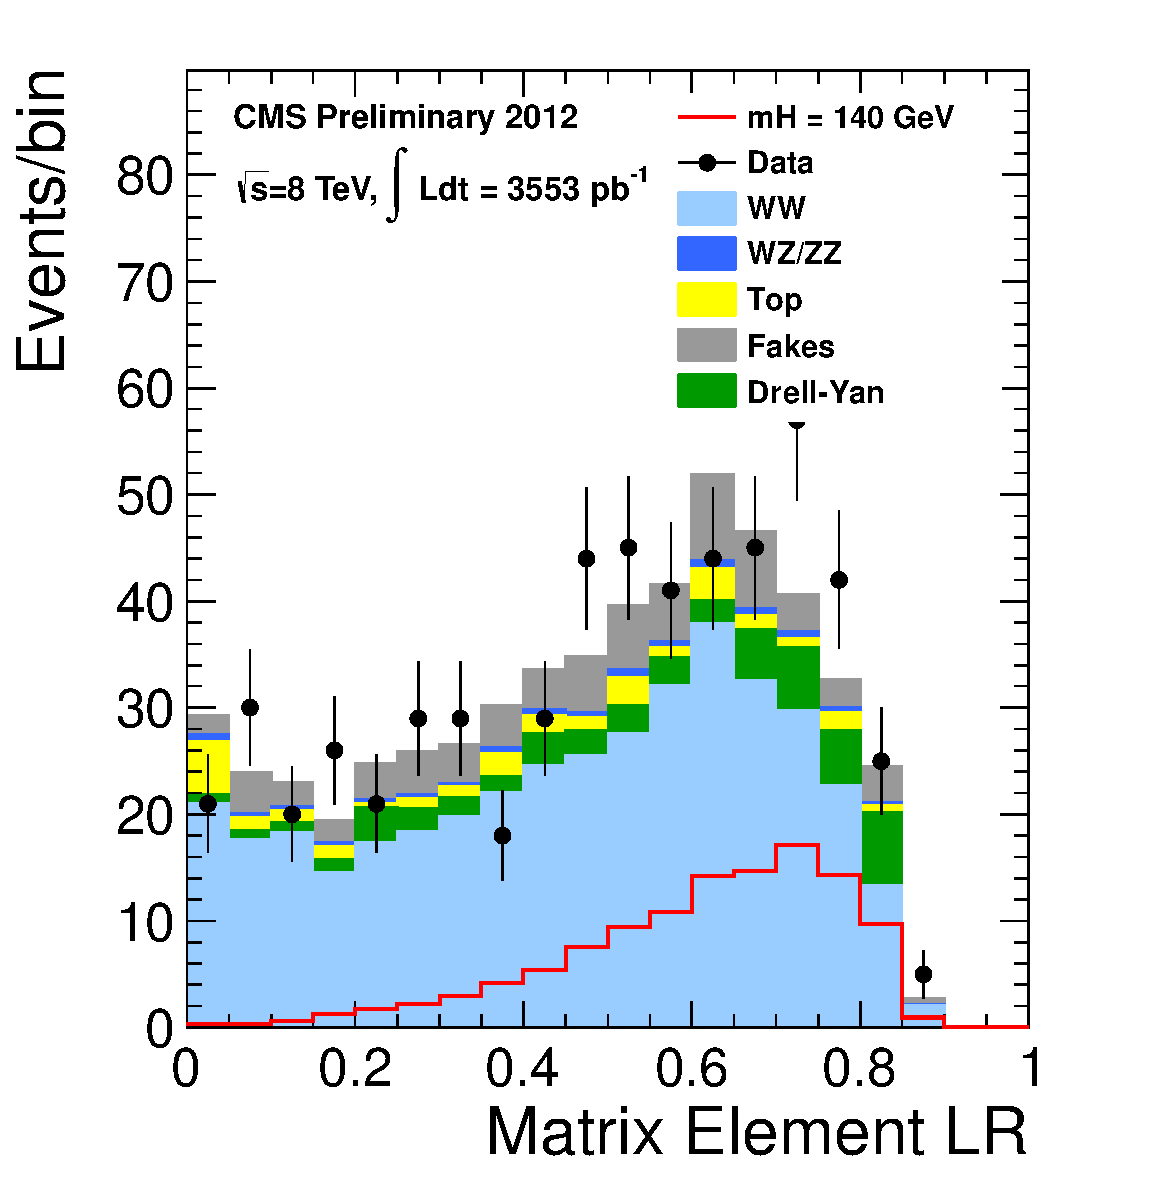
\includegraphics[width=.45\textwidth]{figures/hww_analysis19_140_lr_incl_0j.pdf}}
\subfigure[$mH=150 GeV$]{
\centering
\label{subfig:lr150}
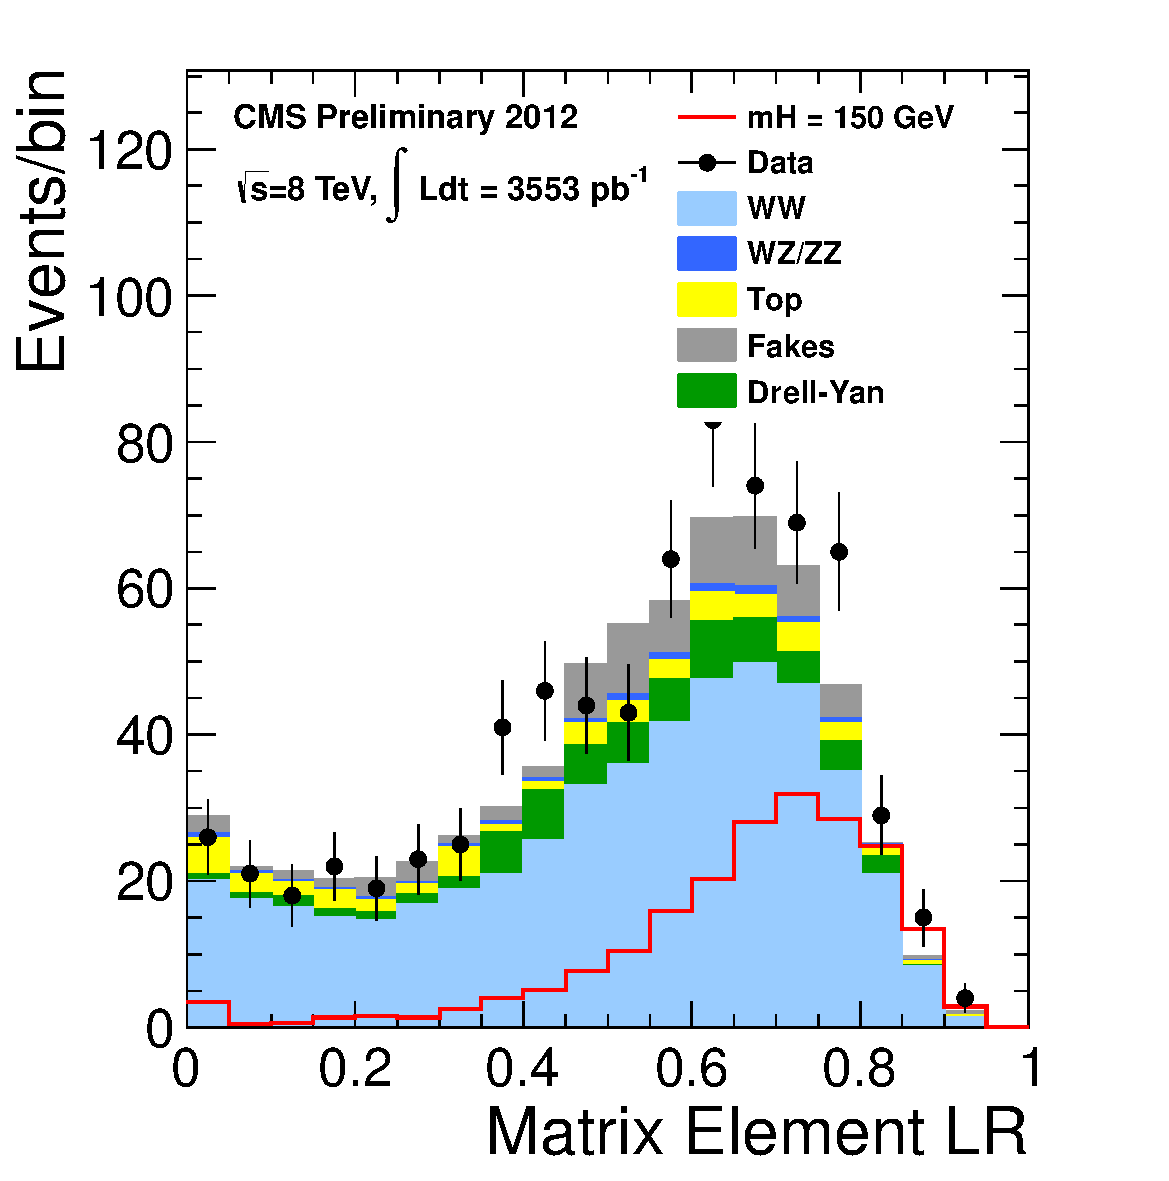
\includegraphics[width=.45\textwidth]{figures/hww_analysis19_150_lr_incl_0j.pdf}}
\caption{Likelihood ratio for Higgs mass hypotheses 140 and 150 \GeV.}
\label{fig:me_lr_140_150}
\end{figure}

\begin{figure}[!hbtp]
\subfigure[$mH=160 GeV$]{
\centering
\label{subfig:lr160}
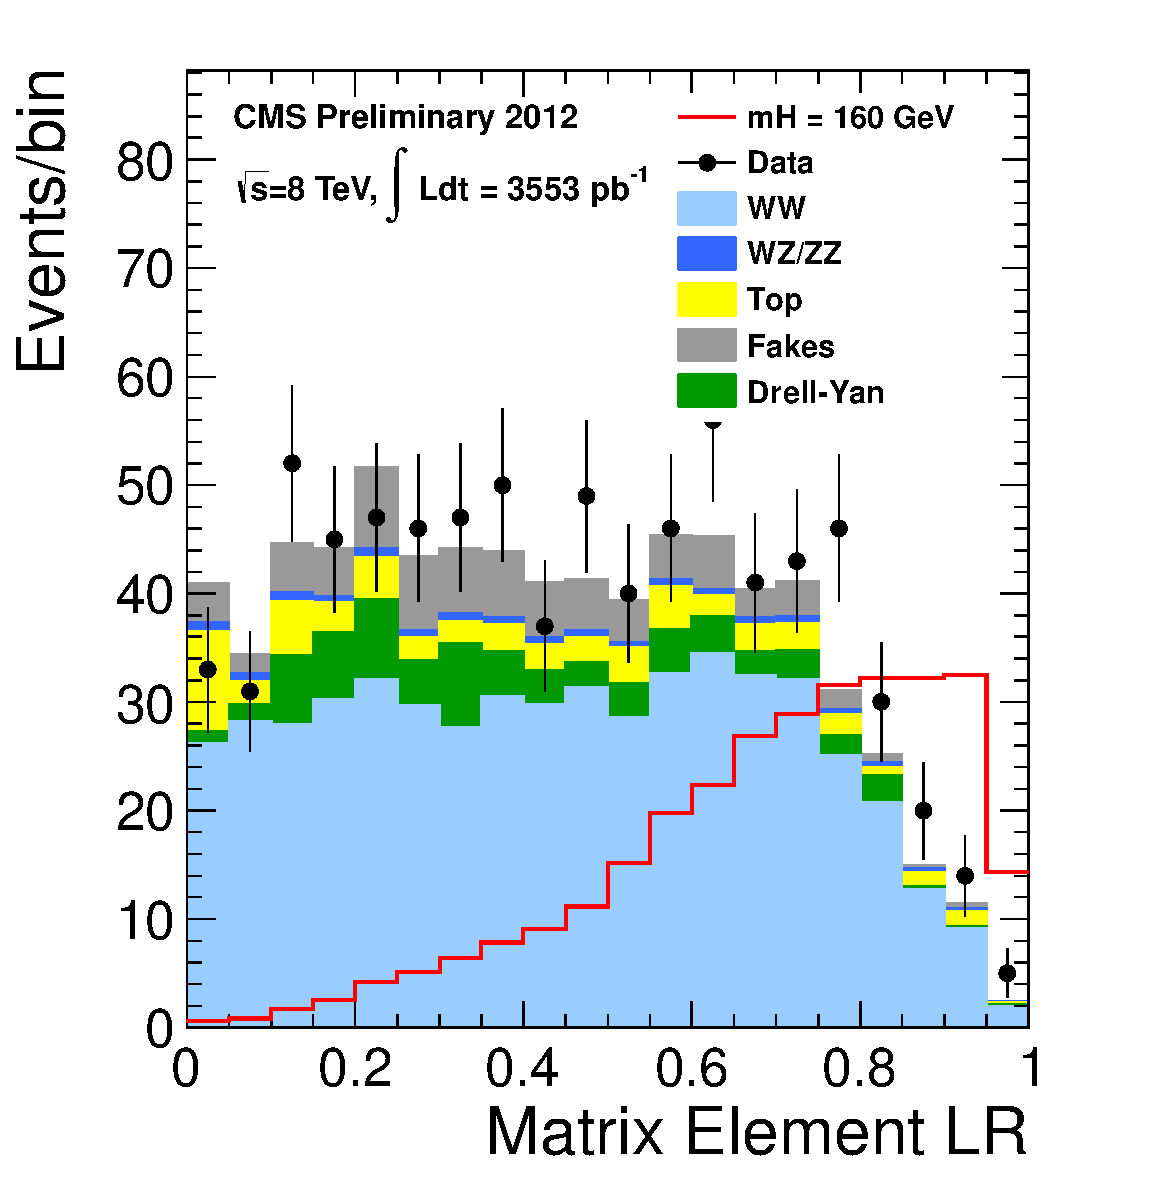
\includegraphics[width=.45\textwidth]{figures/hww_analysis19_160_lr_incl_0j.pdf}}
\subfigure[$mH=200 GeV$]{
\centering
\label{subfig:lr200}
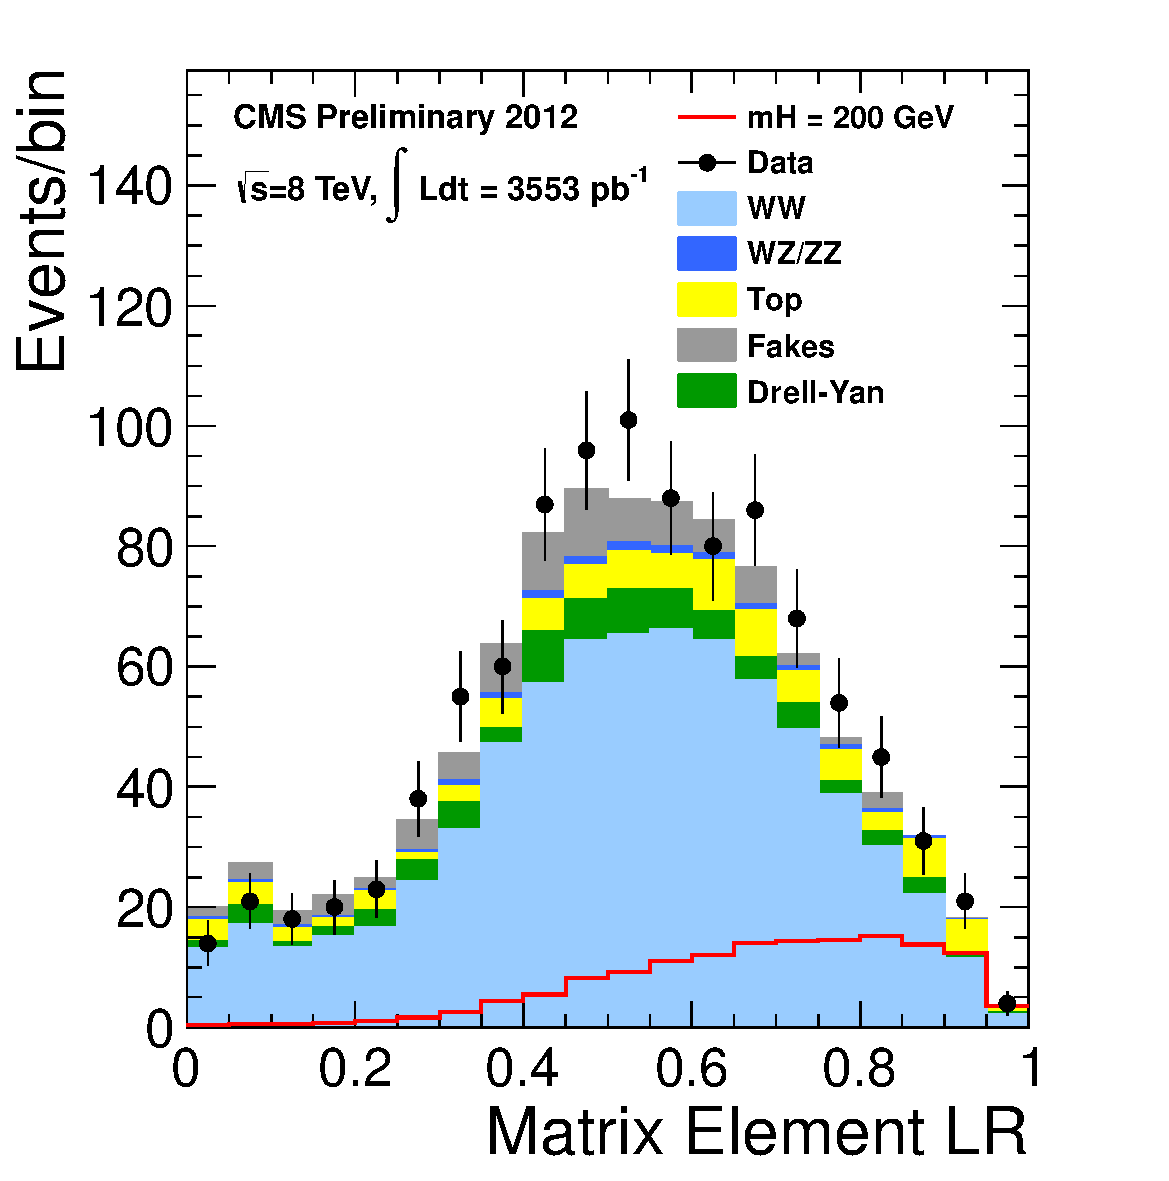
\includegraphics[width=.45\textwidth]{figures/hww_analysis19_200_lr_incl_0j.pdf}}
\caption{Likelihood ratio for Higgs mass hypotheses 160 and 200 \GeV.}
\label{fig:me_lr_160_200}
\end{figure}

%%%%%%%%%%%%%%%%%%%%%%

\subsection{Correlation between likelihood ratio and BDT output}

In this section we examine the correlation
between the matrix element LR discriminator 
and the BDT output.  
To do this, we select events in the samples of simulated
Higgs boson decays with $m_{H}=125 \GeV$ and
simulated $qq\rightarrow WW$ decays, using the standard
BDT analysis preselection in the zero jet bin.
The data are selected in the same way.
We then calculate the correlation co-efficients 
between the two discriminators, and between each
discriminator and relevant kinematic variables.

We observe the correlation co-efficient between the
matrix element LR discriminator and the BDT output to be $0.66$ in the 
signal sample and $0.78$ in the background sample.
While the matrix element and the BDT have similar
expected sensitivity to the Higgs boson signal, they are not
$100\%$ correlated.  This means that the matrix element
discrimnator can be used to provide a partially independent
cross check of the BDT based analysis.

The correlation co-efficients between the
two discriminating variables, and the event kinematic variables
are given in Table \ref{tab:bdt_me_correlations} using the simulated samples.
We observe that the value of both discriminators is highly
correlated with $M_{ll}$, however less so for the 
matrix element than the BDT.

The correlation between the output of the two discriminators
is shown for the data and the expected signal and background
in Figures \ref{fig:me_correlations_all}, 
\ref{fig:me_correlations_sf} and \ref{fig:me_correlations_of}.
The output assigned to data events in both discriminators
is qualitatively consistent with expectations.
Signal like events have a high score in both discriminators,
and background like events have a low score in both discriminators.

\vspace{30pt}
\begin{table}[ht!]
\begin{center}
\begin{tabular}{l|c|c}
\hline
Variable        &   Signal Events   & Background Events \\ \hline
\hline
\multicolumn{3}{c}{Matrix Element LR} \\
\hline

$p_{T} (trail)$ &   -0.508485       &  -0.553587 \\
$M_{ll}$        &   -0.489669       &  -0.709396 \\
$p_{T} (lead)$  &   -0.327346       &  -0.306577 \\
$M_{T}$         &   -0.270782       &  -0.212003 \\
$MET$           &  -0.247144        &  -0.201313 \\
$\Delta\phi$    &   -0.170118       &  -0.310511  \\
\hline
\multicolumn{3}{c}{BDT} \\
\hline
$M_{ll}$        &  -0.738705       &  -0.873989 \\
$p_{T} (trail)$ &  -0.55488        &  -0.542548 \\
$\Delta\phi$    &  -0.403576       &  -0.510162  \\
$M_{T}$         &  -0.2568         &  -0.266183  \\
$p_{T} (lead)$  &  -0.217102       &  -0.342558 \\
$MET$           &  -0.138572       &  -0.156602 \\
\hline
\end{tabular}
\end{center}
\caption{ The correlations of the matrix element LR and BDT discriminators, with
event kinematic variables in simulated events.  Rows are sorted by highest correlation in signal events. }
\label{tab:bdt_me_correlations}
\end{table}

\begin{figure}[!hbtp]
\centering
\subfigure[$m_{H}=125$~GeV]{\label{subfig:fig_me_correlations_s}
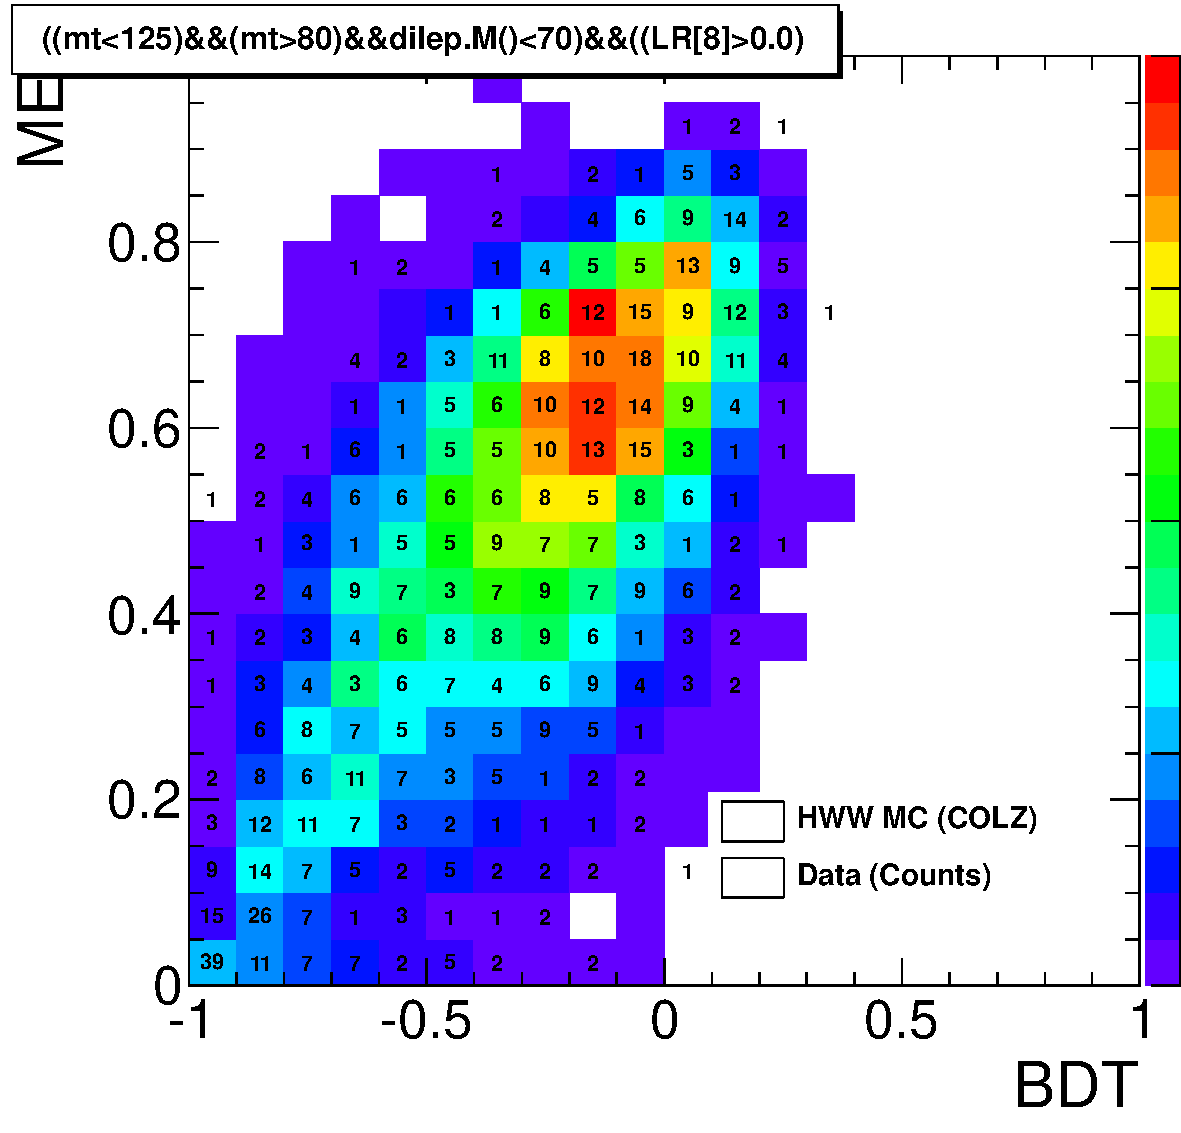
\includegraphics[width=.45\textwidth]{figures/bdt_me_hww125_all.pdf}}
\subfigure[$qq\rightarrow WW$]{\label{subfig:fig_me_correlations_b}
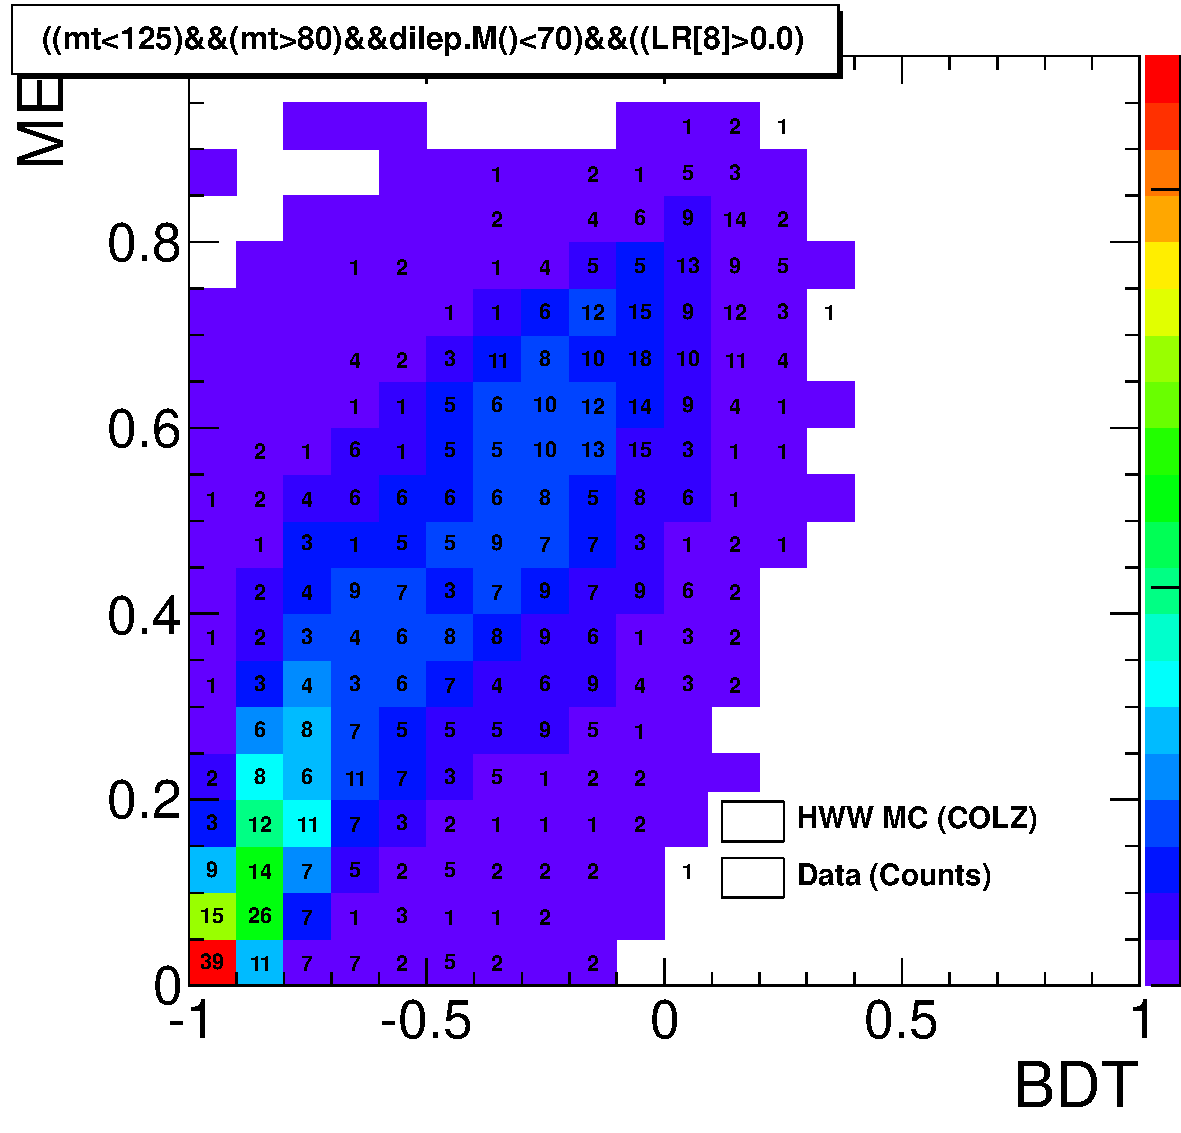
\includegraphics[width=.45\textwidth]{figures/bdt_me_qqww_all.pdf}}
\caption{Correlation between BDT and ME LR in data
and simulated $qq\rightarrow WW$ and $m_{H}=125$~GeV decays.
Events are shown in all lepton channels.  Correlation is $0.66$ for signal and $0.78$ for background.}.
\label{fig:me_correlations_all}
\end{figure}

\begin{figure}[!hbtp]
\centering
\subfigure[$m_{H}=125$~GeV]{\label{subfig:fig_me_correlations_s}
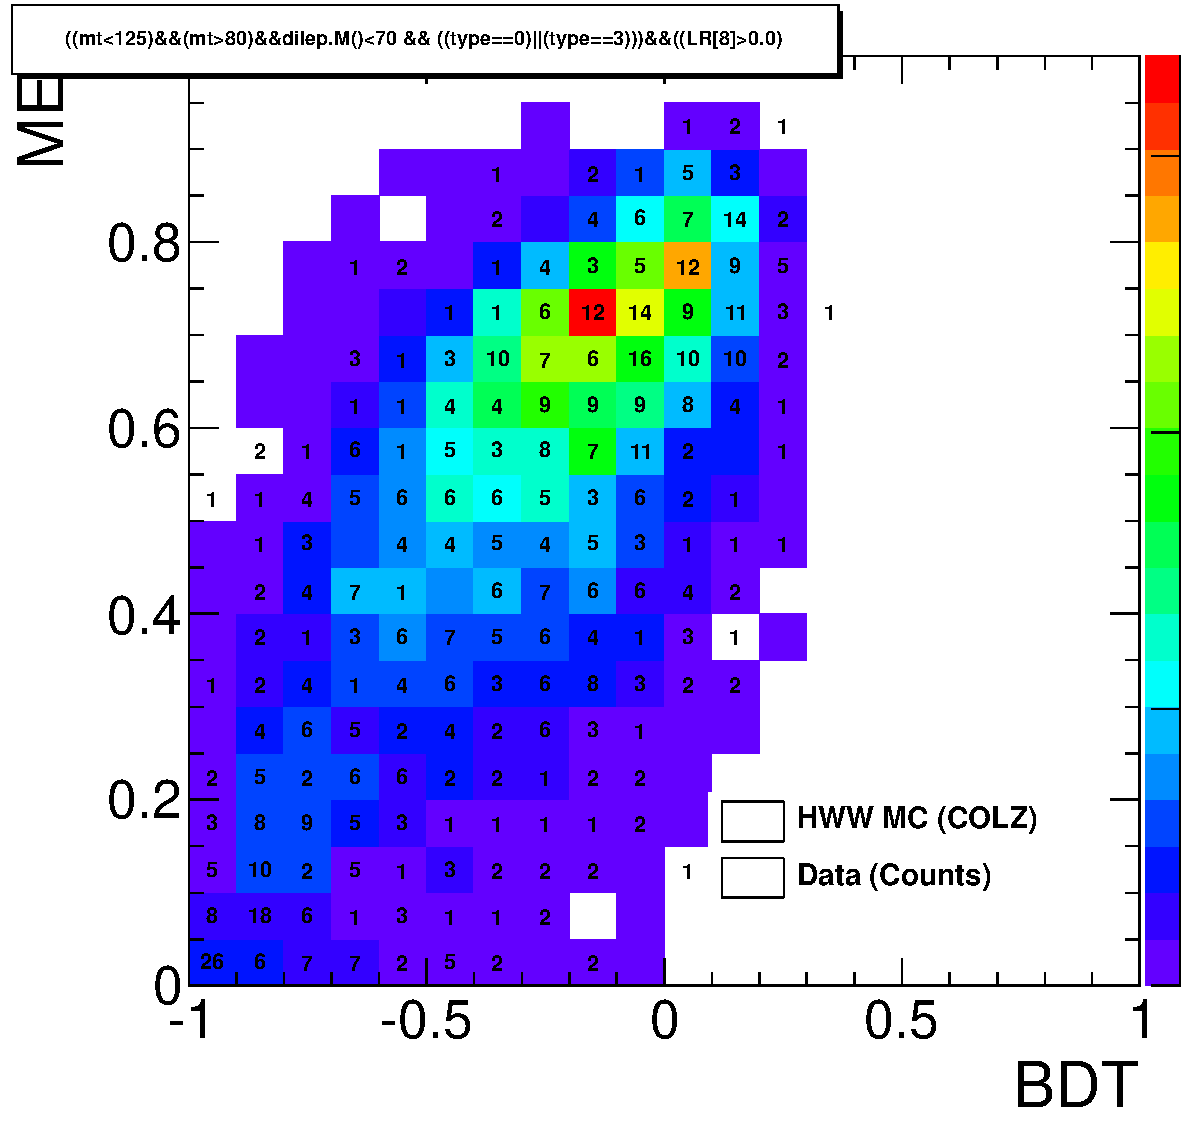
\includegraphics[width=.45\textwidth]{figures/bdt_me_hww125_sf.pdf}}
\subfigure[$qq\rightarrow WW$]{\label{subfig:fig_me_correlations_b}
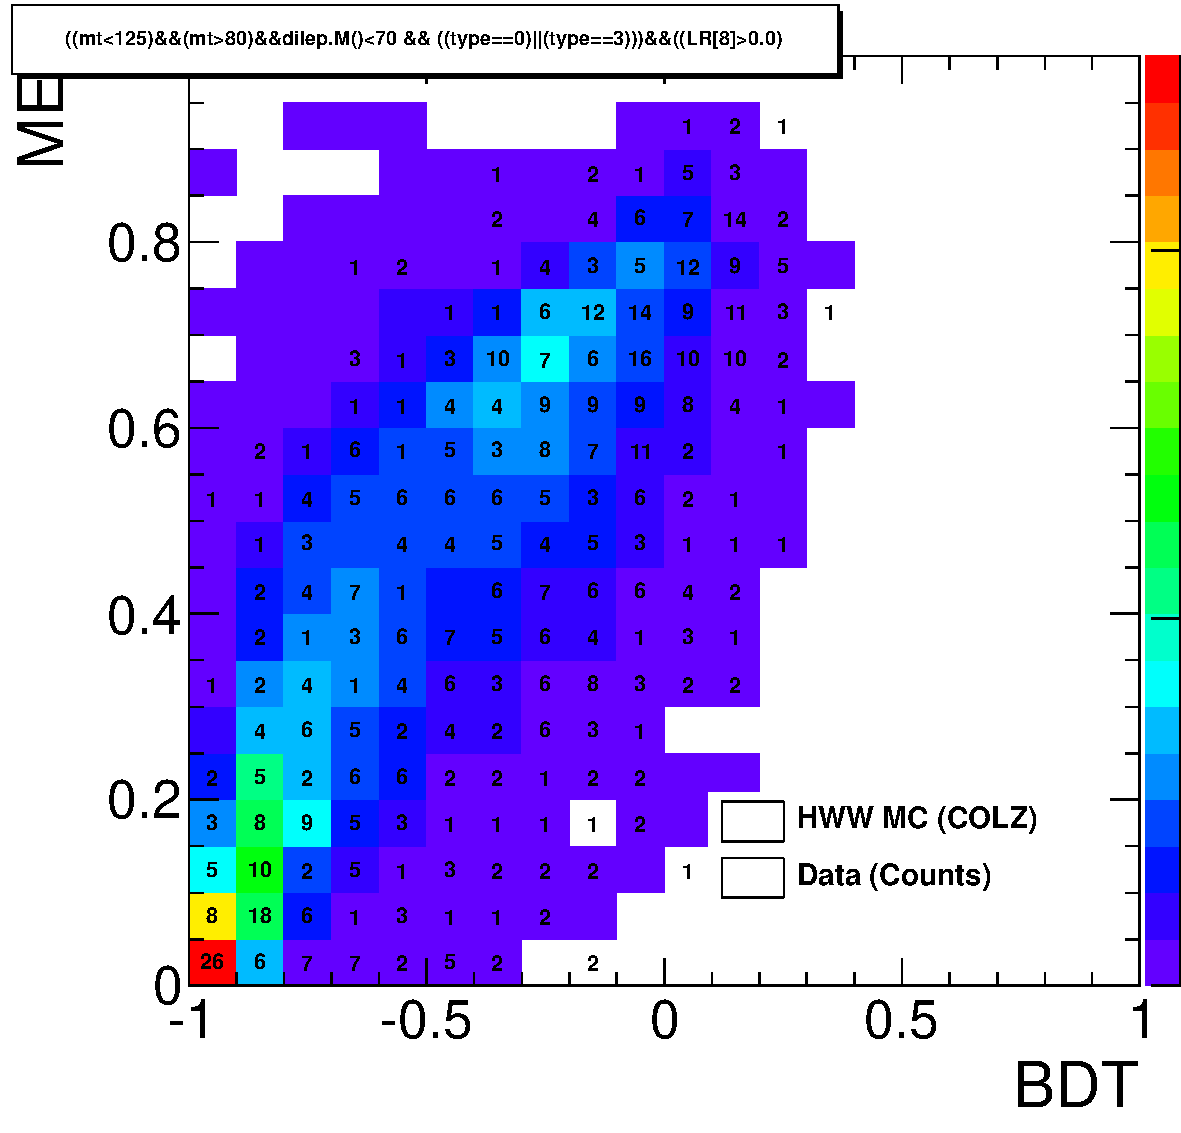
\includegraphics[width=.45\textwidth]{figures/bdt_me_qqww_sf.pdf}}
\caption{Correlation between BDT and ME LR in data
and simulated $qq\rightarrow WW$ and $m_{H}=125$~GeV decays.
Events are shown in the $\mu\mu$ and $ee$ channels. Correlation is $0.66$ for signal and $0.79$ for background.}
\label{fig:me_correlations_sf}
\end{figure}

\begin{figure}[!hbtp]
\centering
\subfigure[$m_{H}=125$~GeV]{\label{subfig:fig_me_correlations_s}
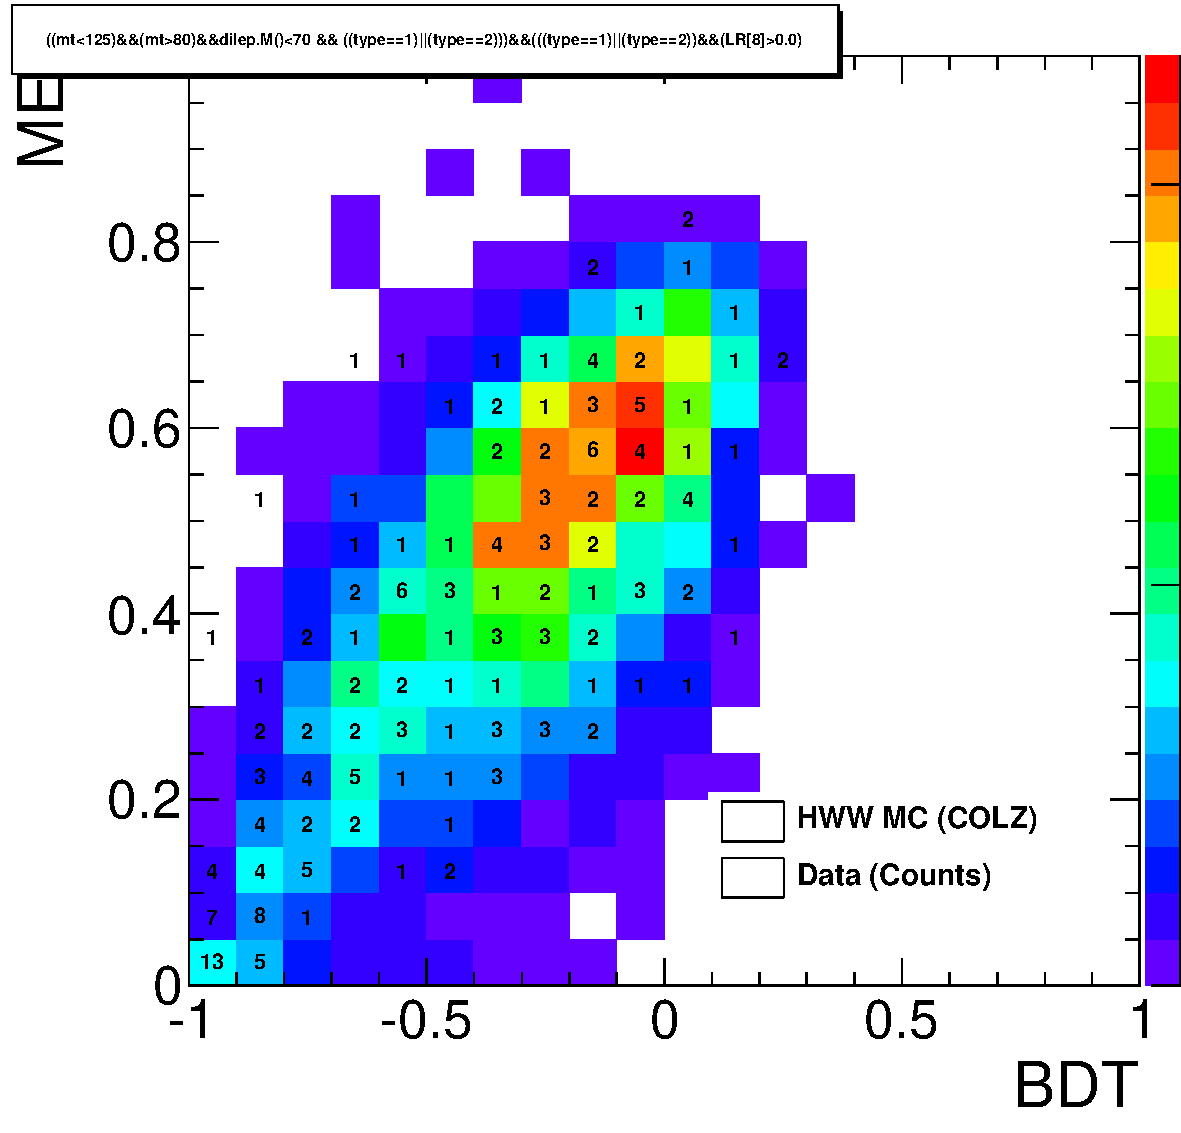
\includegraphics[width=.45\textwidth]{figures/bdt_me_hww125_of.pdf}}
\subfigure[$qq\rightarrow WW$]{\label{subfig:fig_me_correlations_b}
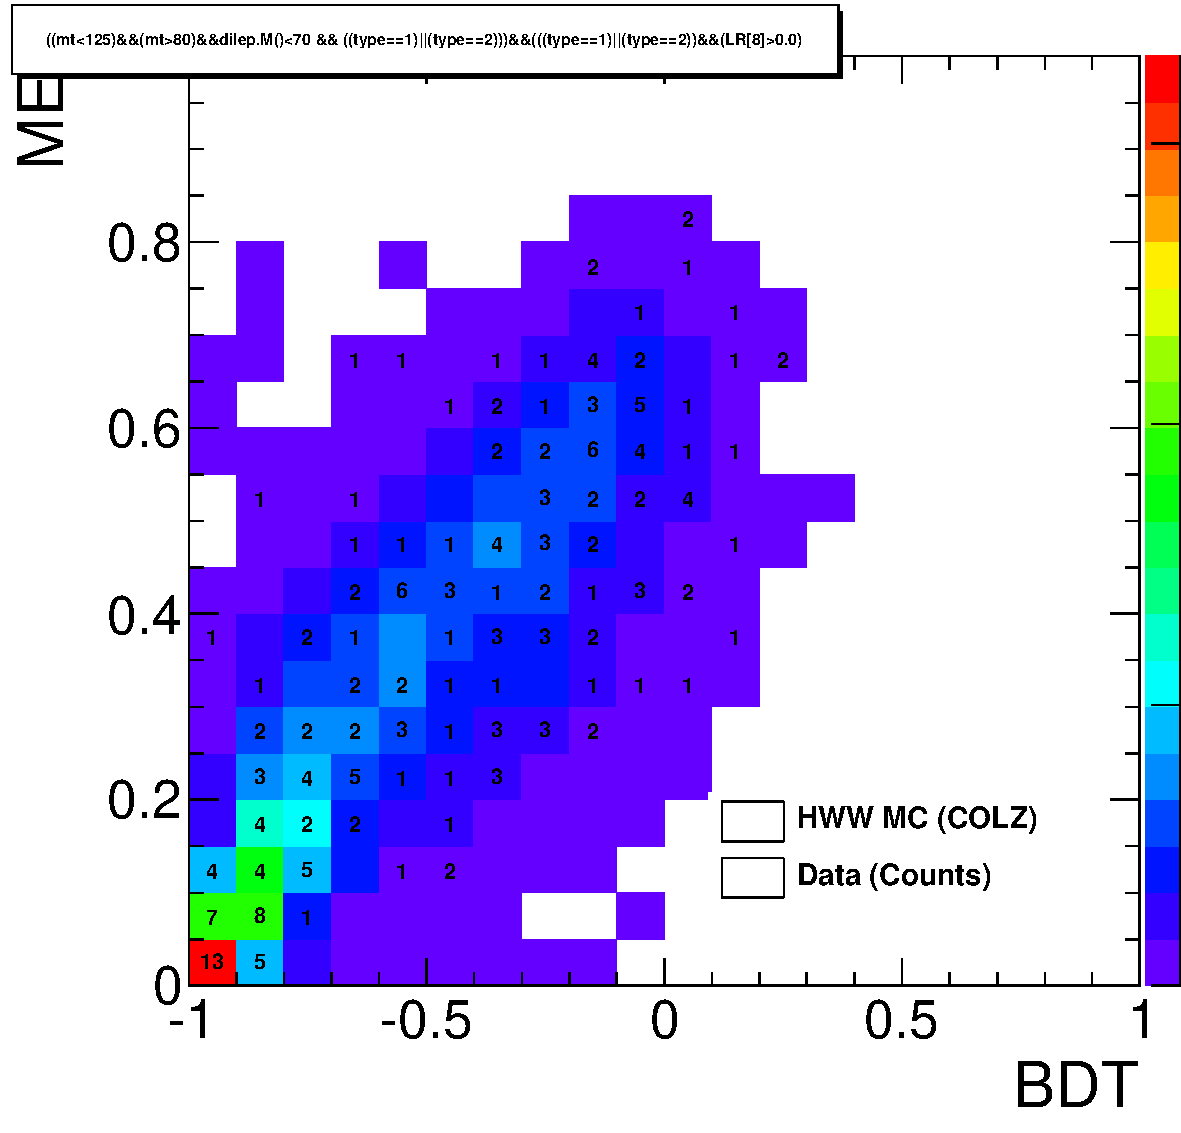
\includegraphics[width=.45\textwidth]{figures/bdt_me_qqww_of.pdf}}
\caption{Correlation between BDT and ME LR in data
and simulated $qq\rightarrow WW$ and $m_{H}=125$~GeV decays.
Events are shown in the $e\mu$ and $\mu e$ channels. Correlation is $0.69$ for signal and $0.80$ for background.}
\label{fig:me_correlations_of}
\end{figure}


\clearpage

